\documentclass[10pt,conference]{IEEEtran}
\usepackage{amsmath, amssymb}
\usepackage{tikz}
\usetikzlibrary{calc}

\begin{document}

    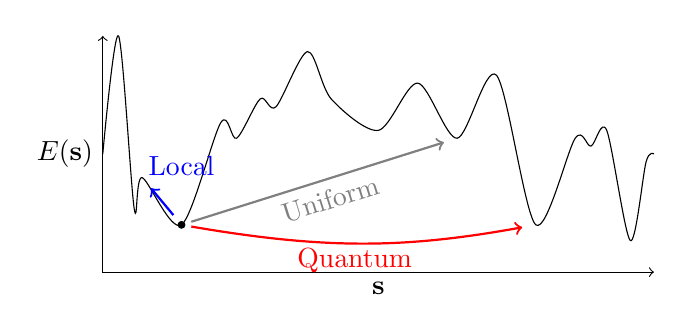
\begin{tikzpicture}

\draw[<->] (0,3)  -- node[left]{$E(\mathbf{s})$} (0,0) -- node[below] {$\mathbf{s}$} (7,0) ;
\draw plot[smooth] coordinates {(0,1.5) (.2, 3) (.4, .8) (.5, 1.2) (1, 0.6) (1.5, 1.9) (1.7, 1.7) (2, 2.2) (2.2, 2.1) (2.6, 2.8) (2.9, 2.2) (3.5, 1.8) (4,2.4) (4.5, 1.7) (5, 2.5) (5.5, .6) (6, 1.7) (6.2, 1.6) (6.4, 1.8) (6.7, .4) (6.9, 1.4) (7,1.5)};
\fill (1, .6) circle (.05) node (local) {};
\node at (local) [above = .5cm, blue] {Local};
\draw[->, shorten > = 5pt, blue, thick] (local) -- (.5, 1.2);
\draw[->, shorten > = 5pt, gray, thick] (local) -- (4.5, 1.7) node[midway, below, sloped] {Uniform};
\draw[->, shorten > = 5pt, red, thick] (local) to[bend right=10] (5.5, .6);
\draw(3.2, .15) node[red] {Quantum};

\end{tikzpicture}

\end{document}